% Provenance (never printed): see sources/outline_sources.md (Year 3:
% Darcy's law; permeability; aquifer types; the groundwater-flow equation;
% pumping tests; solute transport, in principle).
% Brief: sources/book5/BRIEFS.md, ch. 23. Curves from figdata/bachelor-3/
% theis.py, flow_net.py and advection_dispersion.py; the site of Varden-3 from
% figdata/shared/region.py (read only). Exercise and problem values in the
% Book 5 scratch calculator calc/ch23.py. The wells, the dam, the tests and
% the solutes are invented.
\chapter{Hydrogeologie}\label{ch:b3:hydrogeology}

Een nieuwe put pompt dagelijks \qty{2160}{m^3} water op uit een kalksteenlaag
enkele honderden meter onder een boerderij. Aan de eigen put van die boerderij gebeurt
aanvankelijk niets. Een maand later staat het water daarin bijna \qty{2}{m} lager, hoewel
die put een kilometer verderop ligt en het pompstation er nog nooit een druppel uit heeft gehaald. De
waterstand rond de nieuwe put is niet gelijkmatig gedaald: ze is in een kegel weggezakt,
en die kegel is snel gegroeid door een gesteente waarin het water zelf maar een paar
centimeter per dag beweegt. Dit hoofdstuk bouwt de natuurkunde op die beide getallen
voorspelt, de snelle voortplanting van de druk en de trage verplaatsing van het water,
uit één empirische wet die in 1856 werd gevonden.
% ledger: heath:darcy

\begin{recall}
Porositeit, permeabiliteit, de grondwaterspiegel, grondwater, watervoerende lagen,
bronnen en putten staan in de schoolboeken, samen met de verblijftijd van water en
fossiel grondwater. Viscositeit, de wet van Poiseuille voor de stroming in een buis
en de diffusievergelijking staan in de natuurkundeboeken. De foutenfunctie en
de oplossingen van de diffusievergelijking die daarvan gebruikmaken staan in
Hoofdstuk~\ref{ch:b3:lithosphere-thermal-models}. De Varden Hills, de
verzonnen regio van de serie, met hun zandsteen, kalksteen, schalie en krijt,
zijn sinds de schoolboeken de regio van de oefeningen.
\end{recall}

\section{Stijghoogte en de wet van Darcy}\label{sec:b3:hydrogeology:darcy}

Water in de ondergrond stroomt van waar zijn mechanische energie per gewichtseenheid
hoog is naar waar die lager is. Omdat het langzaam stroomt, is de kinetische energie
verwaarloosbaar, en die energie bestaat uit twee delen: de hoogte van het water en
zijn druk.

\begin{definition}[Stijghoogte; hydraulische gradiënt]\label{def:b3:hydrogeology:head}
De \emph{stijghoogte}\index{stijghoogte} in een punt van de verzadigde
grond is
\[
h = z + \frac{p}{\rho g} ,
\]
de som van de \emph{plaatshoogte} $z$ van het punt boven een referentievlak en
\emph{drukhoogte} $p/(\rho g)$, waarbij $p$ de druk van het water boven de
atmosferische druk is. Het is de hoogte waartoe het water stijgt in een buis,
een piezometer, die alleen op dat punt open is. De \emph{hydraulische
gradiënt}\index{hydraulische gradiënt} is $\nabla h$; de grootte ervan tussen twee
punten op afstand $L$ langs de stroming is $\Delta h/L$.
\end{definition}

\begin{omfigure}
\centering
\begin{tikzpicture}[>=stealth, font=\small, x=1cm, y=1cm]
\fill[omLithAlluv!60] (0,-0.6) rectangle (7,3.2);
\fill[omSea!45] (0,-0.6) rectangle (7,1.9);
\draw[thick, brown!60!black] (0,3.2) -- (7,3.2);
\draw[omDef, dashed] (0,1.9) -- (7,1.9);
\node[omDef, font=\scriptsize, anchor=south east] at (6.9,1.92) {grondwaterspiegel};
% piezometer
\fill[white] (3.3,0.4) rectangle (3.7,4.0);
\draw[thick] (3.3,0.7) -- (3.3,4.0); \draw[thick] (3.7,0.7) -- (3.7,4.0);
\draw[thick, densely dotted] (3.3,0.4) -- (3.3,0.7); \draw[thick, densely dotted] (3.7,0.4) -- (3.7,0.7);
\fill[omSea!70] (3.32,0.4) rectangle (3.68,2.6);
\draw[omDef, thick] (3.3,2.6) -- (3.7,2.6);
\fill (3.5,0.55) circle (0.06);
\node[font=\scriptsize, anchor=west] at (3.75,0.55) {filter, in het punt $P$};
% datum
\draw[black!60] (0,-0.6) -- (7,-0.6);
\node[font=\scriptsize, anchor=north west] at (0,-0.62) {referentievlak, $z = 0$};
% heads, on the left of the tube
\draw[<->] (2.5,-0.6) -- node[left, font=\scriptsize] {$z$} (2.5,0.55);
\draw[<->] (2.5,0.55) -- node[left, font=\scriptsize] {$p/\rho g$} (2.5,2.6);
\draw[black!40, densely dashed] (2.4,0.55) -- (3.3,0.55);
\draw[black!40, densely dashed] (1.0,2.6) -- (3.3,2.6);
\draw[<->, thick, omThm] (1.1,-0.6) -- node[left, font=\scriptsize] {$h$} (1.1,2.6);
\node[font=\scriptsize, anchor=south] at (3.5,4.0) {piëzometer};
\end{tikzpicture}

\par\smallskip{\small Een piezometer, een buis die alleen bij zijn filter open is. Het
water staat erin op de \omterm{def:b3:hydrogeology:head}{stijghoogte} van het punt $P$: de plaatshoogte $z$
plus de drukhoogte. Hier ligt het niveau in de buis boven de
grondwaterspiegel, zoals het doet waar het water opstijgt naar een bron of een
rivier.}\label{fig:b3:hydrogeology:head}
\end{omfigure}

In 1856 mat Henry Darcy, een Franse ingenieur, de stroming van water door
kolommen zand en vond dat die evenredig is met het verlies aan \omterm{def:b3:hydrogeology:head}{stijghoogte} per
eenheid van lengte. De stroming is laminair: het water volgt afzonderlijke stroomlijnen.
% ledger: heath:darcy

\begin{theorem}[Wet van Darcy]\label{thm:b3:hydrogeology:darcy}
In een verzadigd poreus medium is het volume water dat per
tijdseenheid door een eenheid van oppervlakte stroomt, gelijk aan
\[
\vec q = -K\,\nabla h ,
\]
waarbij $K$ afhangt van het medium en van de vloeistof. In een medium waarvan de poriën
evenwijdige rechte buizen met straal $a$ zijn die een fractie $n$ van het
volume innemen, geeft de wet van Poiseuille deze wet met
\[
K = \frac{k\rho g}{\mu}, \qquad k = \frac{na^2}{8} ,
\]
waarbij $\mu$ de viscositeit van het water is.
\end{theorem}
\index{wet van Darcy}

\begin{proof}
Het eerste deel van de bewering is de empirische \omterm{thm:b3:hydrogeology:darcy}{wet van Darcy}. In een buis met straal $a$
langs de stroming geeft de wet van Poiseuille de gemiddelde snelheid $\bar u =
-(a^2/8\mu)\,\mathrm d(p + \rho gz)/\mathrm dl = -(a^2\rho g/8\mu)\,\mathrm
dh/\mathrm dl$, omdat $p + \rho gz = \rho g h$. De buizen beslaan de
fractie $n$ van elke doorsnede, dus het volume per eenheid van totaal oppervlak is
$q = n\bar u = -(na^2/8)(\rho g/\mu)\,\mathrm dh/\mathrm dl$.
\end{proof}

Echte poriën zijn geen rechte buizen; de stelling toont de vorm van de wet
en hoe die schaalt. De stroming is evenredig met de gradiënt, met het kwadraat
van de grootte van de poriën, en omgekeerd evenredig met de viscositeit: hetzelfde zand
laat water sneller door als het warm is.

\begin{definition}[Specifiek debiet; hydraulische geleidbaarheid; intrinsieke permeabiliteit]\label{def:b3:hydrogeology:darcy}
Het \emph{specifiek debiet}\index{specifiek debiet} $\vec q$ is het
volume water dat per eenheid van oppervlak door het medium stroomt, korrels en poriën
samen, per tijdseenheid. De \emph{hydraulische
geleidbaarheid}\index{hydraulische geleidbaarheid} $K$ is de coëfficiënt
van de \omterm{thm:b3:hydrogeology:darcy}{wet van Darcy}, in \unit{m/s} of \unit{m/d}. De \emph{intrinsieke
permeabiliteit}\index{intrinsieke permeabiliteit} van het medium is $k =
K\mu/(\rho g)$, in \unit{m^2}: zij hangt alleen van het medium af.
\end{definition}

De \omterm{def:b3:hydrogeology:darcy}{hydraulische geleidbaarheid} van gesteenten bestrijkt twaalf ordes van grootte,
zoals weinig fysische grootheden dat doen. Af te lezen aan de grafiek van een klassiek
overzichtsonderzoek van het onderwerp zijn de gangbare bereiken, in meter per dag, als volgt: klei
\num{e-7} tot \num{e-4}; silt en löss \num{e-3} tot 2; zandig silt 0.04 tot
10; schoon zand 0.3 tot 150; grind 100 tot 4000; schalie \num{e-8} tot
\num{e-4}; zandsteen \num{e-5} tot 0.4; carbonaatgesteenten \num{e-4} wanneer ze
alleen gebroken zijn tot enkele duizenden wanneer ze holend zijn; stollingsgesteenten en
metamorfe gesteenten onder \num{e-8} wanneer ongebroken tot enkele wanneer
gebroken. De meeste gesteenten geleiden water ook beter langs hun gelaagdheid dan
dwars erop.
% ledger: heath:darcy, heath:k-chart

Het \omterm{def:b3:hydrogeology:darcy}{specifiek debiet} is een flux door het hele oppervlak; het water stroomt
alleen door de poriën, en sneller.

\begin{definition}[Poriesnelheid]\label{def:b3:hydrogeology:seepage}
De \emph{poriesnelheid}\index{poriesnelheid} is $\vec v = \vec
q/n_e$, de gemiddelde snelheid van het water in de poriën, waarbij $n_e$ de
effectieve porositeit is, die van de verbonden poriën waardoor het water
stroomt.
\end{definition}

Een grof zand met $K = \qty{60}{m/d}$, een gradiënt van 1 op 1000 en een
porositeit van 0.20 laat het water er met \qty{0.3}{m/d} stromen; een klei met $K =
\qty{e-4}{m/d}$, een gradiënt van 1 op 10 en een porositeit van 0.50, bij
\qty{2e-5}{m/d}, minder dan een centimeter per jaar. Grondwater stroomt niet
in ondergrondse rivieren, behalve in de grotten van kalksteen en de buizen
van lava. Dit zijn gemiddelden: waar een verontreiniging zich verplaatst, kan het
snelste deel ervan enkele keren sneller gaan.
% ledger: heath:velocity

\section{Watervoerende lagen}\label{sec:b3:hydrogeology:aquifers}

\begin{definition}[Freatische en gespannen watervoerende lagen; aquitard]\label{def:b3:hydrogeology:aquifer-types}
Een \emph{freatische watervoerende laag}\index{freatische watervoerende laag} is een watervoerende laag waarvan het
bovenvlak de grondwaterspiegel is. Een \emph{gespannen
watervoerende laag}\index{gespannen watervoerende laag} is een watervoerende laag die wordt afgedekt door een laag met veel
lagere geleidbaarheid, zodat het water erin onder druk staat: in een put die
ze bereikt, stijgt het water boven de bovenkant van de watervoerende laag,
tot aan het potentiometrisch oppervlak. Een laag met lage geleidbaarheid die de
doorstroming van water tussen watervoerende lagen vertraagt maar niet stopt, is een
\emph{aquitard}\index{aquitard}.
\end{definition}

\begin{definition}[Transmissiviteit; bergingscoëfficiënt; specifieke berging]\label{def:b3:hydrogeology:storage}
De \emph{transmissiviteit}\index{transmissiviteit} van een watervoerende laag met dikte
$b$ is $T = Kb$, de stroming per eenheid van breedte onder eenheidsgradiënt, in
\unit{m^2/d}. De \emph{bergingscoëfficiënt}\index{bergingscoëfficiënt} (ook wel
storage coefficient) $S$ is het volume water dat per eenheid van oppervlak van de
watervoerende laag vrijkomt wanneer de \omterm{def:b3:hydrogeology:head}{stijghoogte} met één eenheid daalt; zij is dimensieloos. De
\emph{specifieke berging}\index{specifieke berging} $S_y$ van een gesteente is het
volume water dat per eenheid van volume door de zwaartekracht uit het gesteente
wegloopt wanneer de grondwaterspiegel erdoor zakt.
\end{definition}

De twee soorten watervoerende lagen geven water op verschillende manieren vrij. In een \omterm{def:b3:hydrogeology:aquifer-types}{gespannen
watervoerende laag} daalt de \omterm{def:b3:hydrogeology:head}{stijghoogte}, maar blijven de poriën vol: het water zet
iets uit, en de watervoerende laag, die meer van het gewicht van de gesteenten
erboven draagt, wordt iets samengedrukt. De uitzetting van het water alleen geeft
ongeveer \num{9e-7} kubieke meter per kubieke meter watervoerende laag en per meter
\omterm{def:b3:hydrogeology:head}{stijghoogte} vrij; met de samendrukking ligt de \omterm{def:b3:hydrogeology:storage}{bergingscoëfficiënt} van de meeste
gespannen watervoerende lagen tussen \num{e-5} en \num{e-3}. In een \omterm{def:b3:hydrogeology:aquifer-types}{freatische
watervoerende laag} daalt de grondwaterspiegel en lopen de poriën erboven leeg:
de \omterm{def:b3:hydrogeology:storage}{bergingscoëfficiënt} is de \omterm{def:b3:hydrogeology:storage}{specifieke berging}, ongeveer 0.1 tot 0.3, honderd
tot tienduizend keer groter. De \omterm{def:b3:hydrogeology:storage}{transmissiviteiten} van de in gebruik zijnde watervoerende lagen
lopen uiteen van minder dan \qty{1}{m^2/d} in gebroken gesteenten tot
\qty{100000}{m^2/d} in holle kalksteen en lavastromen. Wanneer de \omterm{def:b3:hydrogeology:head}{stijghoogte} van een \omterm{def:b3:hydrogeology:aquifer-types}{gespannen
watervoerende laag} lange tijd wordt verlaagd, lopen de kleilagen erin en eromheen leeg en drukken ze samen, en het maaiveld erboven zakt.
% ledger: heath:storage, heath:transmissivity

\begin{omfigure}
\centering
\begin{tikzpicture}[>=stealth, font=\small, x=1cm, y=1.1cm]
\begin{scope}
\clip (0,-1.3) -- (0,2.0) -- (3.5,2.9) -- (5,3.5) -- (7.5,4.2) -- (11,3.8) -- (11,-1.3) -- cycle;
\fill[lith sandstone] (0,-1.3) rectangle (11,4.5);
\fill[lith limestone] (0,1.8) -- (11,-0.95) -- (11,0.05) -- (0,2.8) -- cycle;
\fill[lith shale] (0,2.8) -- (11,0.05) -- (11,1.25) -- (0,4.0) -- cycle;
\fill[omLithLime!25] (0,4.0) -- (11,1.25) -- (11,4.5) -- (0,4.5) -- cycle;
\end{scope}
\draw[thick, brown!60!black] (0,2.0) -- (3.5,2.9) -- (5,3.5) -- (7.5,4.2) -- (11,3.8);
% water table in the chalk
\draw[omDef, dashed, thick] (4.5,3.0) .. controls (6,3.35) and (8.5,3.35) .. (11,2.8);
\node[omDef, font=\scriptsize, anchor=south] at (6.6,3.32) {grondwaterspiegel};
% potentiometric surface of the limestone
\draw[omThm, densely dashdotted, thick] (1.4,2.36) -- (11,2.2);
\node[omThm, font=\scriptsize, anchor=south east, fill=white, inner sep=1pt] at (10.9,2.25) {potentiometrisch oppervlak van de kalksteen};
% well Varden-3
\draw[thick] (2.9,2.74) -- (2.9,1.05); \draw[thick] (3.1,2.8) -- (3.1,1.05);
\fill[omDef!35] (2.92,1.05) rectangle (3.08,2.33);
\draw[omThm, thick] (2.85,2.33) -- (3.15,2.33);
\node[font=\scriptsize, anchor=south] at (3.0,2.95) {Varden-3};
% labels
\node[font=\scriptsize, fill=white, inner sep=1pt] at (7.5,0.45) {kalksteen: gespannen watervoerende laag};
\node[font=\scriptsize, fill=white, inner sep=1pt] at (7.5,1.5) {schalie: afdeklaag};
\node[font=\scriptsize, fill=white, inner sep=1pt] at (8.4,2.8) {krijt: freatische watervoerende laag};
\node[font=\scriptsize, fill=white, inner sep=1pt] at (7.5,-0.8) {zandsteen};
\node[font=\scriptsize, fill=white, inner sep=1pt, align=center] at (0.8,1.75) {kalksteen\\ontsluiting};
\draw[->, omDef, thick] (0.8,3.0) -- (0.8,2.3);
\node[omDef, font=\scriptsize, anchor=south] at (0.8,3.0) {voeding};
\end{tikzpicture}

\par\smallskip{\small Een schematische doorsnede van de deklaag van de Varden Hills
van west naar oost, niet op schaal. De krijt bevat een \omterm{def:b3:hydrogeology:aquifer-types}{freatische watervoerende laag}
onder de grondwaterspiegel. De Jurassische kalksteen wordt gevoed waar hij
ontsloten is en is gespannen onder de schalie: in de put Varden-3 uit het
probleem, geboord door de schalie en alleen open naar de kalksteen, stijgt het
water tot het potentiometrisch oppervlak, ver boven de bovenkant van de
watervoerende laag maar onder het maaiveld.}\label{fig:b3:hydrogeology:aquifers}
\end{omfigure}
% ledger: region:name

\section{De grondwaterstromingsvergelijking}\label{sec:b3:hydrogeology:flow-equation}

\begin{theorem}[Grondwaterstromingsvergelijking]\label{thm:b3:hydrogeology:flow-equation}
In een \omterm{def:b3:hydrogeology:aquifer-types}{gespannen watervoerende laag} met constante \omterm{def:b3:hydrogeology:storage}{transmissiviteit} $T$ en \omterm{def:b3:hydrogeology:storage}{bergingscoëfficiënt} $S$,
met horizontale stroming voldoet de \omterm{def:b3:hydrogeology:head}{stijghoogte} $h(x, y, t)$ aan
\[
S\,\frac{\partial h}{\partial t} = T\nabla^2h + W ,
\]
$W$ is het volume water dat per oppervlakte-eenheid en tijdseenheid door voeding wordt toegevoegd of
door pompen wordt onttrokken (negatief). Bij stationaire stroming zonder bronnen geldt $\nabla^2h =
0$.
\end{theorem}
\index{grondwaterstromingsvergelijking}

\begin{proof}
Neem een kolom van de watervoerende laag met oppervlak $\mathrm dx\,\mathrm dy$. De stroming per
eenheid van breedte over de volle dikte is $-T\nabla h$, volgens de \omterm{thm:b3:hydrogeology:darcy}{wet van Darcy}
vermenigvuldigd met $b$. De netto instroom is $-\nabla\cdot(-T\nabla h)\,\mathrm dx\,\mathrm
dy = T\nabla^2h\,\mathrm dx\,\mathrm dy$. Het in de kolom opgeslagen water
verandert met de snelheid $S\,(\partial h/\partial t)\,\mathrm dx\,\mathrm dy$,
volgens de definitie van $S$. Massabehoud, waarbij de dichtheid van het water constant
wordt verondersteld in de balans, stelt de opslag gelijk aan instroom plus bronnen.
\end{proof}

Het is de diffusievergelijking uit de natuurkundeboeken, met de hydraulische
diffusiviteit $T/S$ in plaats van een thermische. Voor een gespannen kalksteen met
$T = \qty{450}{m^2/d}$ en $S = \num{2e-4}$ bedraagt de diffusiviteit
\qty{2.25e6}{m^2/d}: een verandering van de \omterm{def:b3:hydrogeology:head}{stijghoogte} verspreidt zich over \qty{1}{km} in
ongeveer $L^2S/T$, een halve dag. Dezelfde kalksteen, freatisch, met $S =
0.2$, zou duizend keer zo lang duren. De druk verspreidt zich snel, het water
beweegt langzaam: de twee getallen van de opening.

\begin{proposition}[Stationaire radiale stroming naar een put]\label{prop:b3:hydrogeology:thiem}
Een put pompt $Q$ uit een \omterm{def:b3:hydrogeology:aquifer-types}{gespannen watervoerende laag} met \omterm{def:b3:hydrogeology:storage}{transmissiviteit} $T$, waarbij de
stroming stationair en radiaal is. Tussen twee afstanden $r_1 < r_2$ van de put verschillen de
verlagingen met
\[
s_1 - s_2 = \frac{Q}{2\pi T}\ln\frac{r_2}{r_1} .
\]
\end{proposition}

\begin{proof}
Door elke cirkel met straal $r$ rond de put is de instroom $Q = 2\pi r
T\,\mathrm dh/\mathrm dr$. Integreren van $\mathrm dh = (Q/2\pi T)\,\mathrm
dr/r$ van $r_1$ tot $r_2$, en met $s = h_0 - h$ geeft het resultaat.
\end{proof}

In twee dimensies wordt stationaire stroming getekend met een \omterm{def:b3:hydrogeology:flow-net}{stroomnet}.

\begin{definition}[Stroomnet]\label{def:b3:hydrogeology:flow-net}
Een \emph{stroomnet}\index{stroomnet} is een tekening van stationaire grondwaterstroming in
een homogene, isotrope doorsnede door twee families van krommen: equipotentiaallijnen,
lijnen van gelijke \omterm{def:b3:hydrogeology:head}{stijghoogte}, en stroomlijnen, die het water volgt. De
stroomlijnen snijden de equipotentiaallijnen loodrecht, en in een stroomnet liggen
ze zo dat de cellen krommlijnige vierkanten zijn.
\end{definition}

\begin{method}[Kwel uit een stroomnet]\label{met:b3:hydrogeology:flow-net}
\leavevmode
\begin{enumerate}
\item Teken de randen: een ondoorlatende rand is een stroomlijn; de bodem van een
  waterlichaam, waar de \omterm{def:b3:hydrogeology:head}{stijghoogte} vastligt, is een equipotentiaallijn.
\item Teken $N_d$ stijghoogteverschillen tussen de hoogste en laagste \omterm{def:b3:hydrogeology:head}{stijghoogte}, $\Delta h
  = H/N_d$, en de stroomlijnen die $N_f$ stroombanen vormen, door proberen,
  totdat elke cel een krommlijnig vierkant is.
\item Elke stroombaan voert $K\Delta h$ per eenheid van lengte loodrecht op de
  doorsnede, waarbij de lengte en breedte van het vierkant wegvallen: het totaal is $q =
  KHN_f/N_d$.
\end{enumerate}
\end{method}

\begin{omfigure}
\centering
\begin{tikzpicture}
\begin{axis}[width=0.95\linewidth, height=0.36\linewidth, axis equal image,
  xmin=-60, xmax=60, ymin=-20, ymax=13, xlabel={$x$ (\unit{m})}, ylabel={$z$ (\unit{m})},
  tick label style={font=\scriptsize}, label style={font=\small}, clip=false]
% computed in figdata/bachelor-3/flow_net.py
\fill[omLithAlluv!35] (axis cs:-60,-20) rectangle (axis cs:60,0);
\fill[omSea!40] (axis cs:-60,0) rectangle (axis cs:-10,11.2);
\fill[omSea!40] (axis cs:10,0) rectangle (axis cs:60,1.2);
\fill[black!35] (axis cs:-10,0) -- (axis cs:-10,12.5) -- (axis cs:-5,12.5) -- (axis cs:10,0) -- cycle;
\pgfplotsinvokeforeach{1,...,9}{
  \addplot[omThm, thin, unbounded coords=jump] table[x=x, y=z] {figdata/out/bachelor-3-flow_net-h-#1.dat};}
\pgfplotsinvokeforeach{1,...,4}{
  \addplot[omMeth, thick, unbounded coords=jump] table[x=x, y=z] {figdata/out/bachelor-3-flow_net-psi-#1.dat};}
\draw[very thick] (axis cs:-60,-20) -- (axis cs:60,-20);
\node[font=\scriptsize, anchor=south] at (axis cs:45,-19.6) {ondoorlatend gesteente};
\node[font=\scriptsize, align=center] at (axis cs:-36,6) {reservoir, \qty{10}{m} boven\\het benedenstroomse water};
\node[font=\scriptsize, anchor=south] at (axis cs:35,1.4) {benedenstroomse water};
\node[font=\scriptsize] at (axis cs:-4,4) {dam};
\end{axis}
\end{tikzpicture}

\par\smallskip{\small Kwel onder een dam van \qty{20}{m} breed op een laag
zand van \qty{20}{m} dik, het reservoir \qty{10}{m} boven het water benedenstrooms,
berekend door de Laplace-vergelijking op te lossen voor de \omterm{def:b3:hydrogeology:head}{stijghoogte} en voor de
stroomfunctie. Dunne lijnen: equipotentiaallijnen, één per meter \omterm{def:b3:hydrogeology:head}{stijghoogte}. Dikke
lijnen: vier stroomlijnen die, samen met de basis van de dam en de vloer,
vijf stroombanen begrenzen. De berekende kwel is $0.51\,KH$ per meter
dam; het \omterm{def:b3:hydrogeology:flow-net}{stroomnet} geeft $KH \times 5/10 = 0.50\,KH$.}\label{fig:b3:hydrogeology:flow-net}
\end{omfigure}

\section{Pompproeven}\label{sec:b3:hydrogeology:pumping}

Stationaire stroming naar een put komt zelden voor: een nieuwe stationaire toestand kan maanden of
jaren op zich laten wachten, of komt nooit. In 1935 gaf Theis, van de United States Geological
Survey, de stijghoogteverlaging rond een put die met een constant debiet werd leeggepompt als
functie van de tijd; uit een test van enkele uren of dagen volgen de \omterm{def:b3:hydrogeology:storage}{transmissiviteit} en de
\omterm{def:b3:hydrogeology:storage}{bergingscoëfficiënt} van de watervoerende laag.
% ledger: heath:theis

\begin{theorem}[Theis-oplossing]\label{thm:b3:hydrogeology:theis}
Een put die een oneindige, homogene, \omterm{def:b3:hydrogeology:aquifer-types}{gespannen watervoerende laag} volledig doorboort, met
\omterm{def:b3:hydrogeology:storage}{transmissiviteit} $T$ en \omterm{def:b3:hydrogeology:storage}{bergingscoëfficiënt} $S$, begint op $t = 0$ met pompen tegen het
constante debiet $Q$. De stijghoogteverlaging op afstand $r$ is
\[
s(r, t) = \frac{Q}{4\pi T}\,W(u), \qquad u = \frac{r^2S}{4Tt}, \qquad
W(u) = \int_u^\infty\frac{\mathrm e^{-y}}{y}\,\mathrm dy = -\gamma - \ln u +
u - \frac{u^2}{2\cdot2!} + \frac{u^3}{3\cdot3!} - \cdots,
\]
met $\gamma = \num{0.5772}$. $W$ heet de putfunctie.
\end{theorem}
\index{Theis-oplossing}

\begin{proof}
In radiale vorm luidt de stromingsvergelijking $S\,\partial s/\partial t =
T\,r^{-1}\partial_r(r\,\partial_rs)$, met $s = 0$ op $t = 0$, $s \to 0$ voor
$r \to \infty$ en $2\pi rT\,\partial_rs \to -Q$ voor $r \to 0$. Geen van de
gegevens bevat op zichzelf een lengte of een tijd, dus probeer $s = f(u)$ met $u =
r^2S/4Tt$. Omdat $\partial_ru = 2u/r$ en $\partial_tu = -u/t$, geldt $r\,\partial_rs =
2uf'$, $r^{-1}\partial_r(r\,\partial_rs) = (4u/r^2)(uf')'$ en $\partial_ts =
-(u/t)f'$. Door de vergelijking te vermenigvuldigen met $r^2/(4Tu)$ blijft $(uf')' = -uf'$:
met $g = uf'$, $g' = -g$ en $g = c\,\mathrm e^{-u}$. De putvoorwaarde, $2\pi T\cdot2uf' \to -Q$ voor $u \to 0$, geeft $c =
-Q/4\pi T$, en $f(\infty) = 0$ geeft $f(u) = (Q/4\pi T)\int_u^\infty
\mathrm e^{-y}y^{-1}\,\mathrm dy$. De reeks volgt uit
$W(u) = -\gamma - \ln u + \int_0^u(1 - \mathrm e^{-y})\,y^{-1}\,\mathrm dy$,
waarbij de constante van Euler is, door term voor term te integreren.
\end{proof}

\begin{proposition}[Cooper--Jacob-benadering]\label{prop:b3:hydrogeology:cooper-jacob}
Voor $u \le 0.05$ ligt de stijghoogteverlaging volgens Theis dicht bij
\[
s = \frac{2.3\,Q}{4\pi T}\log_{10}\frac{2.25\,Tt}{r^2S} :
\]
uitgezet tegen $\log_{10}t$ is de stijghoogteverlaging een rechte lijn waarvan de stijging per
logaritmische cyclus, $\Delta s$, $T = 2.3\,Q/(4\pi\Delta s)$ geeft, en waarvan
het snijpunt met $s = 0$, op $t_0$, $S = 2.25\,Tt_0/r^2$ geeft.
\end{proposition}
\index{Cooper--Jacob-benadering}

\begin{proof}
Voor kleine $u$ geldt $W \approx -\gamma - \ln u = \ln(\mathrm
e^{-\gamma}/u) = \ln(0.5615\cdot4Tt/r^2S) = \ln(2.25\,Tt/r^2S)$; de volgende
term, $u$, is hoogstens \num{0.05}, daar minder dan \qty{2}{\percent} van $W$.
Omdat $\ln x = 2.3\log_{10}x$, stijgt de stijghoogteverlaging met $2.3\,Q/4\pi T$ per
factor tien in tijd, en verdwijnt ze wanneer $2.25\,Tt_0 = r^2S$.
\end{proof}

\begin{omfigure}
\begin{tikzpicture}
\begin{groupplot}[group style={group size=2 by 1, horizontal sep=1.5cm},
  width=0.48\linewidth, height=0.4\linewidth,
  tick label style={font=\scriptsize}, label style={font=\small}, title style={font=\small}]
\nextgroupplot[xmode=log, xlabel={$1/u$}, ylabel={$W(u)$}, xmin=0.1, xmax=1e4, ymin=0, ymax=9,
  title={de putfunctie},
  legend style={font=\scriptsize, at={(0.03,0.97)}, anchor=north west}]
% computed in figdata/bachelor-3/theis.py
\addplot[omDef, thick] table[x=invu, y=W] {figdata/out/bachelor-3-theis-wu.dat};
\addlegendentry{Theis $W(u)$}
\addplot[omThm, densely dashed, thick] table[x=invu, y=Wcj] {figdata/out/bachelor-3-theis-cj.dat};
\addlegendentry{$-\gamma - \ln u$}
\addplot[black!40, densely dotted, forget plot] coordinates {(20,0) (20,9)};
\node[font=\scriptsize, black!60, anchor=west] at (axis cs:24,0.6) {$u = 0.05$};
\nextgroupplot[xmode=log, xlabel={tijd sinds het begin van het pompen (\unit{min})}, ylabel={stijghoogteverlaging (\unit{m})},
  xmin=0.5, xmax=5000, ymin=0, ymax=3.4, title={Varden-3, $r = \qty{60}{m}$},
  legend style={font=\scriptsize, at={(0.03,0.97)}, anchor=north west}]
\addplot[only marks, mark=*, mark size=1.3pt] table[x=tmin, y=s] {figdata/out/bachelor-3-theis-test.dat};
\addlegendentry{gemeten}
\addplot[omMeth, thick, domain=0.973:5000, samples=2] {0.87221*log10(x/0.973132)};
\addlegendentry{Cooper--Jacob-lijn}
\addplot[black!40, densely dotted, forget plot] coordinates {(11.5,0) (11.5,3.4)};
\end{groupplot}
\end{tikzpicture}

\par\smallskip{\small Links de Theis-putfunctie tegen $1/u$ op een
logaritmische as, en haar rechte-lijnbenadering: ze vallen samen zodra $u <
0.05$ (stippellijn). Rechts de stijghoogteverlaging in de waarnemingsput van de
Varden-3-test uit het probleem, \qty{60}{m} van de leegpompte put, en de
rechte lijn die is gefit door de punten na \qty{11.5}{min}, waar $u <
0.05$: de helling geeft $T$, het snijpunt $S$.}\label{fig:b3:hydrogeology:theis}
\end{omfigure}
% ledger: heath:theis, heath:jacob

\begin{definition}[Depressiekegel]\label{def:b3:hydrogeology:cone}
De \emph{depressiekegel}\index{depressiekegel} van een leeggepompte put is
de verlaging van de grondwaterspiegel, of van het potentiometrisch oppervlak,
rond de put; de \omterm{def:b3:hydrogeology:head}{hydraulische gradiënt} wordt steiler richting de put, waardoor al het water
moet passeren.
\end{definition}

Omdat de stijghoogteverlagingen aan een lineaire vergelijking voldoen, tellen de kegels van
meerdere putten op. In een \omterm{def:b3:hydrogeology:aquifer-types}{gespannen watervoerende laag}, met haar kleine \omterm{def:b3:hydrogeology:storage}{bergingscoëfficiënt}, groeit een kegel snel
en lopen de kegels van naburige putten al gauw in elkaar over; in een \omterm{def:b3:hydrogeology:aquifer-types}{freatische
watervoerende laag}, die haar poriën moet leegtrekken, groeit de kegel langzaam. De kegel stopt
pas met groeien wanneer hij voldoende aanvulling heeft opgevangen, of voldoende van de
natuurlijke afvoer van de watervoerende laag naar rivieren en bronnen heeft verminderd, om het
pompen in evenwicht te brengen. Grote onttrekkingen uit een \omterm{def:b3:hydrogeology:aquifer-types}{gespannen watervoerende laag} reiken ver: in 1981
werd ongeveer \qty{277000}{m^3/d} opgepompt uit de watervoerende laag van het Krijt van de
Atlantische kustvlakte, in Virginia en North Carolina, waardoor over het gebied
overlappende kegels waren ontstaan.
% ledger: heath:cone

\begin{omfigure}
\begin{tikzpicture}
\begin{groupplot}[group style={group size=2 by 1, horizontal sep=1.5cm},
  width=0.48\linewidth, height=0.4\linewidth, y dir=reverse,
  tick label style={font=\scriptsize}, label style={font=\small}, title style={font=\small}]
\nextgroupplot[xlabel={afstand tot de put (\unit{m})}, ylabel={verlaging (\unit{m})},
  xmin=0, xmax=3000, ymin=0, ymax=6, title={de depressiekegel van één put},
  scaled x ticks=false, xticklabel style={/pgf/number format/1000 sep={}},
  legend style={font=\scriptsize, at={(0.97,0.03)}, anchor=south east}]
% computed in figdata/bachelor-3/theis.py
\addplot[omThm!50, thick] table[x=r, y=s] {figdata/out/bachelor-3-theis-cone-1.dat};
\addlegendentry{1 dag}
\addplot[omThm!80, thick] table[x=r, y=s] {figdata/out/bachelor-3-theis-cone-10.dat};
\addlegendentry{10 dagen}
\addplot[omThm!60!black, thick] table[x=r, y=s] {figdata/out/bachelor-3-theis-cone-100.dat};
\addlegendentry{100 dagen}
\nextgroupplot[xlabel={$x$ (\unit{m})}, ylabel={verlaging (\unit{m})},
  xmin=-1500, xmax=1900, ymin=0, ymax=9, title={twee putten, 10 dagen},
  scaled x ticks=false, xticklabel style={/pgf/number format/1000 sep={}},
  legend columns=3, legend style={font=\scriptsize, at={(0.5,0.985)}, anchor=north,
  /tikz/every even column/.append style={column sep=3pt}}]
\addplot[omDef, densely dashed] table[x=x, y=s1] {figdata/out/bachelor-3-theis-interf.dat};
\addlegendentry{put bij 0}
\addplot[omMeth, densely dashed] table[x=x, y=s2] {figdata/out/bachelor-3-theis-interf.dat};
\addlegendentry{put bij 400 m}
\addplot[black, thick] table[x=x, y=stot] {figdata/out/bachelor-3-theis-interf.dat};
\addlegendentry{beide}
\end{groupplot}
\end{tikzpicture}

\par\smallskip{\small De \omterm{def:b3:hydrogeology:cone}{Theis-depressiekegel} van de put Varden-3 ($Q =
\qty{2160}{m^3/d}$, $T = \qty{450}{m^2/d}$, $S = \num{2e-4}$), verlaging neerwaarts uitgezet.
Links, na 1, 10 en 100 dagen: de kegel verdiept zich bij elke tienvoudige tijd met hetzelfde bedrag en
verbreedt zich zonder grens in een oneindig uitgestrekte
watervoerende laag. Rechts, twee zulke putten \qty{400}{m} van elkaar na 10 dagen: de
verlagingen tellen op: \qty{5.5}{m} halverwege tussen hen in plaats van \qty{2.7}{m}
voor één put.}\label{fig:b3:hydrogeology:cone}
\end{omfigure}
% ledger: heath:cone, heath:storage

\begin{inthefield}[Een pompproef]
\begin{minipage}[t]{0.55\linewidth}\vspace{0pt}
Vóór een pompproef registreren de hydrogeologen de waterstanden in de
putten een tijdje, om de trend te kennen waarop de proef zal worden gesuperponeerd.
Daarna draait de pomp met een constant debiet, dat stabiel wordt gehouden en gemeten met een
meter op de afvoerleiding, gedurende enkele uren tot enkele dagen. In elke
waarnemingsput, minstens drie daarvan op verschillende afstanden als dat
mogelijk is, wordt de diepte tot het water onder een vast meetpunt op
nauwkeurig bekende tijdstippen afgelezen, veel in de eerste minuten en later minder: met een
gegradueerd stalen meetlint of een elektrisch meetlint waarvan de elektrode een circuit sluit
zodra die het water raakt. Tegenwoordig registreert een in de put gehangen
onderwaterdruksensor, verbonden met een elektronische recorder, de stand bijna
continu.
\end{minipage}\hfill
\begin{minipage}[t]{0.42\linewidth}\vspace{0pt}
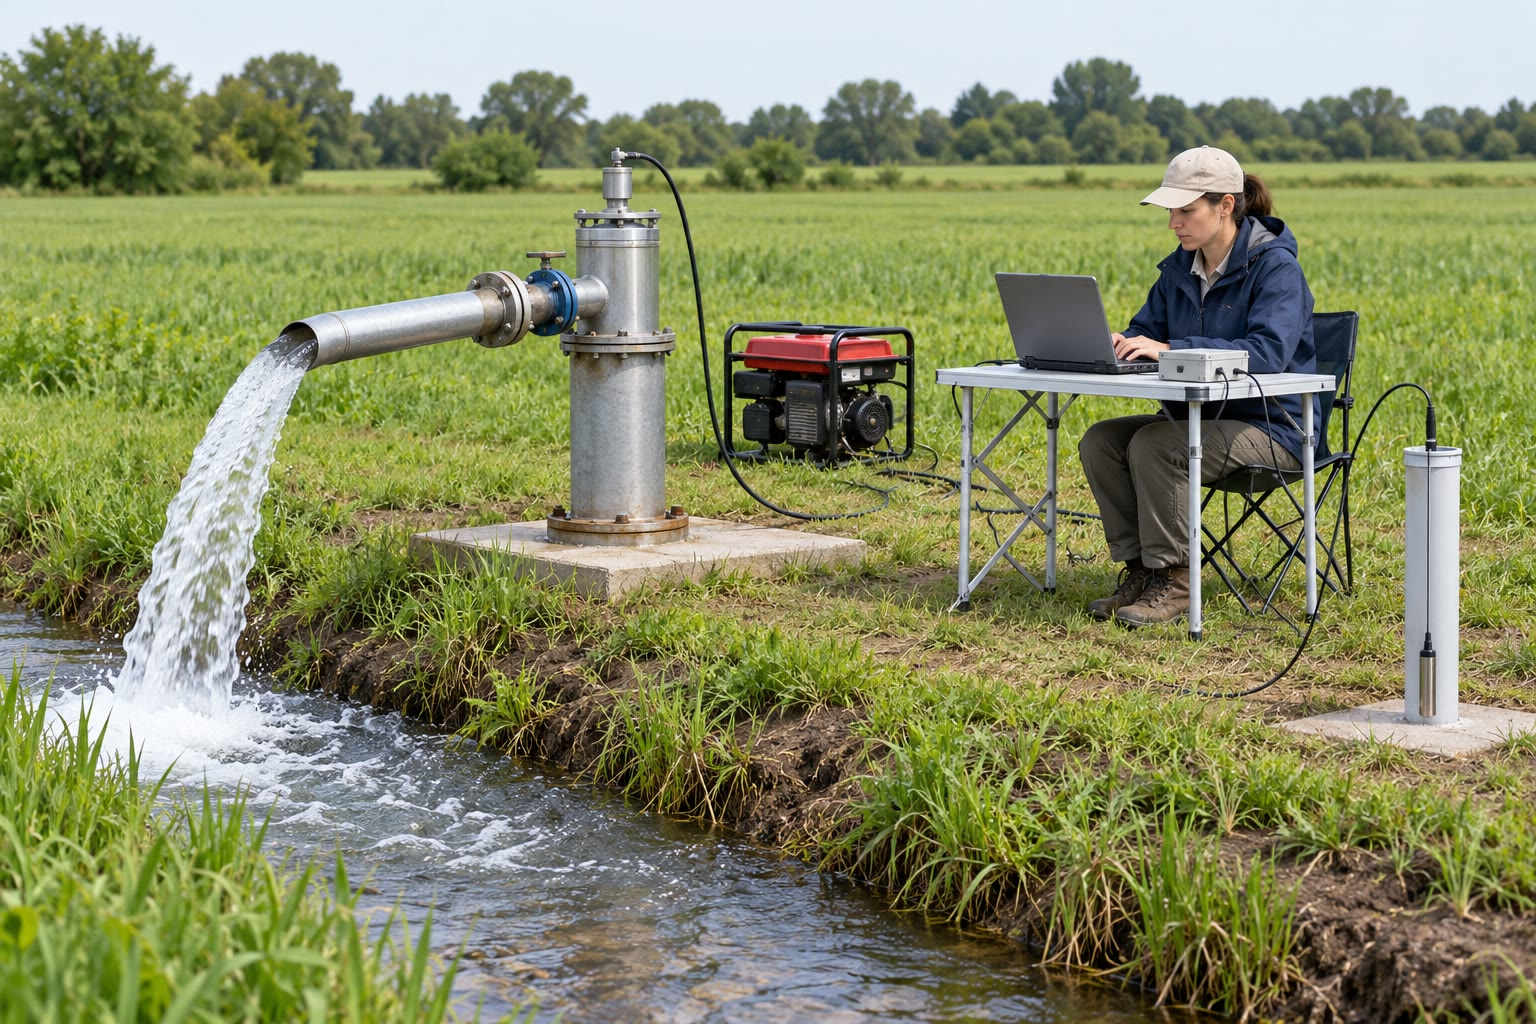
\includegraphics[width=\linewidth]{images/book5/ai/b3-pumping-test.jpg}

{\scriptsize Een pompproef: de afvoerleiding van de gepompte put, een
generator, en een hydrogeoloog die de standen van een waarnemingsput noteert op een
laptop. Door AI gegenereerde illustratie.}
\end{minipage}
\end{inthefield}
% ledger: heath:theis, heath:jacob, heath:water-levels, usgs:transducers

\section{Transport van opgeloste stoffen}\label{sec:b3:hydrogeology:transport}

Een opgeloste stof in grondwater wordt met het water meegevoerd, met de
\omterm{def:b3:hydrogeology:seepage}{poriesnelheid}, en ze spreidt zich onderweg uit: het water in naburige
poriën beweegt met verschillende snelheden en langs verschillende paden, en de stof
diffundeert ook.

\begin{definition}[Hydrodynamische dispersie; dispersiviteit]\label{def:b3:hydrogeology:ade}
\emph{Hydrodynamische dispersie}\index{hydrodynamische dispersie} is het
uitspreiden van een opgeloste stof in stromend grondwater door de variaties in de
snelheid van het water van porie tot porie en door moleculaire diffusie. Langs
de stroming wordt zij beschreven met een dispersiecoëfficiënt $D = \alpha_Lv + D^*$,
$v$ de \omterm{def:b3:hydrogeology:seepage}{poriesnelheid}, $D^*$ de effectieve moleculaire diffusiviteit, en
$\alpha_L$, een lengte, de longitudinale
\emph{dispersiviteit}\index{dispersiviteit} van het medium.
\end{definition}

\begin{theorem}[Advectie--dispersievergelijking]\label{thm:b3:hydrogeology:ade}
Voor een eendimensionale stroming met constante \omterm{def:b3:hydrogeology:seepage}{poriesnelheid} $v$ geldt voor de
concentratie $C(x, t)$ van een niet-reagerende opgeloste stof:
\[
\frac{\partial C}{\partial t} = D\,\frac{\partial^2C}{\partial x^2} -
v\,\frac{\partial C}{\partial x} .
\]
Als de concentratie op $C_0$ wordt gehouden bij $x = 0$ vanaf $t = 0$, in een medium
dat aanvankelijk vrij is van opgeloste stof,
\[
\frac{C}{C_0} = \frac12\left[\operatorname{erfc}\frac{x - vt}{2\sqrt{Dt}} +
\mathrm e^{vx/D}\operatorname{erfc}\frac{x + vt}{2\sqrt{Dt}}\right] .
\]
\end{theorem}
\index{advectie--dispersievergelijking}

\begin{proof}
In een plakje met eenheidsdoorsnede en lengte $\mathrm dx$, met effectieve
porositeit $n_e$, is de opgeslagen hoeveelheid stof $n_eC\,\mathrm dx$. De flux is
$n_e(vC - D\,\partial C/\partial x)$, meegevoerd met het water en verspreid door
dispersie, zoals de wet van Fick een diffunderende stof verspreidt. Massabehoud geeft
$n_e\partial_tC = -\partial_x[n_e(vC - D\partial_xC)]$, de vergelijking. Dat
de formule eraan voldoet en aan de voorwaarden, wordt hier aangenomen;
\cref{exo:b3:hydrogeology:12} toetst de uitspreiding ervan.
\end{proof}

In het met het water meebewegende stelsel, $\xi = x - vt$, is de vergelijking de
diffusievergelijking, en het front verbreedt zich als $\sqrt{2Dt} = \sqrt{2\alpha_L
vt} = \sqrt{2\alpha_Lx}$: de breedte van het front groeit als de wortel
uit de afgelegde afstand.

\begin{definition}[Retardatiefactor]\label{def:b3:hydrogeology:retardation}
Een opgeloste stof die aan de korrels wordt geadsorbeerd, in evenwicht en in verhouding
tot haar concentratie, beweegt langzamer dan het water. Haar
\emph{retardatiefactor}\index{retardatiefactor (sorptie)} is
\[
R = 1 + \frac{\rho_bK_d}{n} ,
\]
waarin $\rho_b$ de droge volumieke dichtheid van het medium is, $n$ de porositeit ervan en
$K_d$ de verdelingscoëfficiënt: de geadsorbeerde massa per eenheid van massa vaste stof
gedeeld door de concentratie in het water. De opgeloste stof beweegt met $v/R$
en disperseert met $D/R$.
\end{definition}

\begin{omfigure}
\begin{tikzpicture}
\begin{groupplot}[group style={group size=2 by 1, horizontal sep=1.5cm},
  width=0.48\linewidth, height=0.4\linewidth,
  tick label style={font=\scriptsize}, label style={font=\small}, title style={font=\small}]
\nextgroupplot[xlabel={tijd (dagen)}, ylabel={$C/C_0$ op \qty{100}{m}},
  xmin=0, xmax=1000, ymin=0, ymax=1.05, title={doorbraakcurven},
  legend style={font=\scriptsize, at={(0.97,0.03)}, anchor=south east}]
% computed in figdata/bachelor-3/advection_dispersion.py
\addplot[omDef, thick] table[x=t, y=c1] {figdata/out/bachelor-3-advection_dispersion-btc.dat};
\addlegendentry{$\alpha_L = \qty{1}{m}$}
\addplot[omMeth, thick] table[x=t, y=c3] {figdata/out/bachelor-3-advection_dispersion-btc.dat};
\addlegendentry{$\alpha_L = \qty{3}{m}$}
\addplot[omThm, thick] table[x=t, y=c10] {figdata/out/bachelor-3-advection_dispersion-btc.dat};
\addlegendentry{$\alpha_L = \qty{10}{m}$}
\addplot[black, thick, densely dashed, forget plot] table[x=t, y=cR] {figdata/out/bachelor-3-advection_dispersion-btc.dat};
\node[font=\scriptsize, anchor=west, align=left] at (axis cs:640,0.45) {$\alpha_L = \qty{3}{m}$,\\ $R = 3$};
\addplot[black!40, densely dotted, forget plot] coordinates {(200,0) (200,1.05)};
\nextgroupplot[xlabel={afstand (\unit{m})}, ylabel={$C/C_0$ na 150 dagen},
  xmin=0, xmax=160, ymin=0, ymax=1.05, title={profielen},
  legend style={font=\scriptsize, at={(0.03,0.03)}, anchor=south west}]
\addplot[omDef, thick] table[x=x, y=c1] {figdata/out/bachelor-3-advection_dispersion-profile.dat};
\addlegendentry{$\alpha_L = \qty{1}{m}$}
\addplot[omMeth, thick] table[x=x, y=c3] {figdata/out/bachelor-3-advection_dispersion-profile.dat};
\addlegendentry{$\alpha_L = \qty{3}{m}$}
\addplot[omThm, thick] table[x=x, y=c10] {figdata/out/bachelor-3-advection_dispersion-profile.dat};
\addlegendentry{$\alpha_L = \qty{10}{m}$}
\addplot[black!40, densely dotted, forget plot] coordinates {(75,0) (75,1.05)};
\end{groupplot}
\end{tikzpicture}

\par\smallskip{\small Een opgeloste stof die continu bij $x = 0$ in een
stroming met een \omterm{def:b3:hydrogeology:seepage}{poriesnelheid} van \qty{0.5}{m/d}. Links, de concentratie
\qty{100}{m} stroomafwaarts als functie van de tijd: het water zelf komt na
200 dagen aan (gestippeld); hoe groter de \omterm{def:b3:hydrogeology:ade}{dispersiviteit}, hoe eerder de eerste
sporen en hoe later de volledige concentratie. Een geadsorbeerde opgeloste stof met $R =
3$ komt drie keer later aan. Rechts, de concentratie langs de stroming na
150 dagen, wanneer het water \qty{75}{m} heeft afgelegd
(gestippeld).}\label{fig:b3:hydrogeology:transport}
\end{omfigure}

\omterm{def:b3:hydrogeology:ade}{Dispersiviteiten} zijn moeilijk te meten, en in de praktijk worden ze vaak vastgelegd met
vuistregels. De oudste neemt de longitudinale \omterm{def:b3:hydrogeology:ade}{dispersiviteit} als een tiende van
de lengte van de pluim. Een compilatie van veldmetingen, gepubliceerd in
1992, laat zien dat de \omterm{def:b3:hydrogeology:ade}{dispersiviteit} groeit met de schaal van het experiment,
dat betrouwbare waarden op grote schaal schaars zijn, en dat op elke schaal de
waarden over twee of drie ordes van grootte verspreid liggen.
% ledger: epa:dispersivity

\section{Oefeningen}

\begin{exercise}[$\star$]\label{exo:b3:hydrogeology:1}
Twee piëzometers staan naast elkaar op maaiveld van \qty{120.0}{m} boven het
referentieniveau. De eerste is gefilterd op \qty{40}{m} diepte en het water staat
\qty{12.5}{m} onder het maaiveld; de tweede is gefilterd op \qty{80}{m}
diepte, met het water \qty{15.0}{m} onder het maaiveld. Bereken de hoogtestijghoogte, de
drukstijghoogte en de \omterm{def:b3:hydrogeology:head}{stijghoogte} op beide filters. In welke richting stroomt het water
tussen hen, en onder welke verticale gradiënt?
\end{exercise}

\begin{exercise}[$\star$]\label{exo:b3:hydrogeology:2}
Een zandkolom van \qty{50}{cm} lang en \qty{10}{cm} in diameter, met $K =
\qty{12}{m/d}$ en een effectieve porositeit van 0.35, laat water door bij een
stijghoogteverschil van \qty{30}{cm}. Bereken het \omterm{def:b3:hydrogeology:darcy}{specifiek debiet}, de doorstroming
in liter per uur, en de \omterm{def:b3:hydrogeology:seepage}{poriesnelheid}.
\end{exercise}

\begin{exercise}[$\star$]\label{exo:b3:hydrogeology:3}
Een kalksteen heeft $K = \qty{2.5}{m/d}$ voor water bij \qty{10}{\celsius}
($\rho = \qty{999.7}{kg/m^3}$, $\mu = \qty{1.306e-3}{Pa.s}$). Bereken de \omterm{def:b3:hydrogeology:darcy}{intrinsieke permeabiliteit} ervan,
en de \omterm{def:b3:hydrogeology:darcy}{hydraulische geleidbaarheid} voor water bij
\qty{20}{\celsius} ($\rho = \qty{998.2}{kg/m^3}$, $\mu =
\qty{1.002e-3}{Pa.s}$).
\end{exercise}
% ledger: nist:water

\begin{exercise}[$\star$]\label{exo:b3:hydrogeology:4}
De gespannen kalksteen van Varden-3 is \qty{180}{m} dik, met $K =
\qty{2.5}{m/d}$. Bereken de \omterm{def:b3:hydrogeology:storage}{transmissiviteit} ervan, en de \omterm{def:b3:hydrogeology:storage}{bergingscoëfficiënt} die hij zou hebben
als alleen de uitzetting van het water, \num{9e-7} per meter watervoerende laag,
per meter \omterm{def:b3:hydrogeology:head}{stijghoogte}, water vrijgaf. Vergelijk met $S = \num{2e-4}$.
\end{exercise}
% ledger: heath:storage

\begin{exercise}[$\star\star$]\label{exo:b3:hydrogeology:5}
Na een lange periode van pompen met \qty{1500}{m^3/d} veranderen de verlagingen
niet meer: \qty{2.35}{m} in een peilbuis op \qty{20}{m} van de pompput en
\qty{0.82}{m} in een peilbuis \qty{200}{m} verderop. De watervoerende laag is
gespannen en \qty{40}{m} dik. Bereken de \omterm{def:b3:hydrogeology:storage}{transmissiviteit} en de \omterm{def:b3:hydrogeology:darcy}{hydraulische
geleidbaarheid}.
\end{exercise}

\begin{exercise}[$\star\star$]\label{exo:b3:hydrogeology:6}
Een put pompt \qty{1200}{m^3/d} uit een \omterm{def:b3:hydrogeology:aquifer-types}{gespannen watervoerende laag} met $T =
\qty{300}{m^2/d}$ en $S = \num{5e-4}$. Bereken $u$, $W(u)$ (uit de
reeks) en de verlaging \qty{300}{m} verderop na 1 dag en na 10 dagen.
\end{exercise}

\begin{exercise}[$\star\star$]\label{exo:b3:hydrogeology:7}
Voor de Varden-3-test ($T = \qty{450}{m^2/d}$, $S = \num{2e-4}$), na
hoeveel minuten mag de Cooper--Jacob-lijn in peilbuizen worden gebruikt
op \qty{60}{m} en \qty{500}{m} van de pompput? Wat zegt dit
over waar de peilbuizen van een korte test moeten staan?
\end{exercise}

\begin{exercise}[$\star\star$]\label{exo:b3:hydrogeology:8}
Twee putten op \qty{400}{m} van elkaar in de Varden-kalksteen pompen elk
\qty{2160}{m^3/d}. Bereken de verlaging na 10 dagen halverwege tussen beide,
en op de locatie van de tweede put ten gevolge van alleen de eerste put. Waarom kost
het pompen van elke put de ander geld?
\end{exercise}

\begin{exercise}[$\star\star$]\label{exo:b3:hydrogeology:9}
Tel in het \omterm{def:b3:hydrogeology:flow-net}{stroomnet} onder de dam de stroombanen en de stijghoogteverschillen.
Bereken met $K = \qty{5}{m/d}$ en $H = \qty{10}{m}$ de kwel per
meter dam en onder een dam van \qty{300}{m} lengte.
\end{exercise}

\begin{exercise}[$\star\star\star$]\label{exo:b3:hydrogeology:10}
Modelleer een schoon zand als rechte buizen met een straal van \qty{50}{\micro\metre} en een
porositeit van 0.30. Bereken $k$ en $K$ (voor water bij \qty{20}{\celsius}, zoals in
\cref{exo:b3:hydrogeology:3}),
en vergelijk met het bereik voor schoon zand. Welke kenmerken van echt zand
laat het model weg, en in welke richting verschuift elk $K$?
\end{exercise}
% ledger: nist:water, heath:k-chart

\begin{exercise}[$\star\star\star$]\label{exo:b3:hydrogeology:11}
(a)~Toon aan dat de verlaging van Cooper--Jacob verdwijnt bij $r_0 =
\sqrt{2.25\,Tt/S}$. (b)~Bereken $r_0$ na 30 dagen pompen in de
gespannen Varden-kalksteen, en voor hetzelfde gesteente als freatische laag, met $S =
0.2$. (c)~Waarom kan de kegel van een \omterm{def:b3:hydrogeology:aquifer-types}{gespannen watervoerende laag} een begrenzing bereiken
die de test niet bedoeld was te zien?
\end{exercise}
% ledger: heath:jacob, heath:storage

\begin{exercise}[$\star\star\star$]\label{exo:b3:hydrogeology:12}
(a)~Bij een grote transportafstand benadert de doorbraakcurve op $x$ een
normale verdeling in de tijd, met gemiddelde $x/v$ en standaardafwijking $\sigma_t
= \sqrt{2\alpha_Lx}/v$. Toon dit aan vanuit de spreiding $\sqrt{2Dt}$ van het front.
(b)~Op \qty{100}{m}, met $v = \qty{0.5}{m/d}$, bereikt de concentratie
\qty{16}{\percent} na \num{152.6}~dagen en \qty{84}{\percent} na
\num{247.2}~dagen. Schat $\alpha_L$. (c)~Een zandige watervoerende laag heeft $\rho_b =
\qty{1.9}{g/cm^3}$ en $n = 0.30$; een opgeloste stof heeft $K_d =
\qty{0.32}{cm^3/g}$. Bereken $R$.
\end{exercise}

\section{Probleem: Pompproef bij Varden-3}

\begin{problem}[{Weekendprobleem --- stijghoogten, een pompproef en het transport van
een verontreinigende stof in de gespannen kalksteen van de Varden Hills}]
\label{pb:b3:hydrogeology:1}
De fictieve put Varden-3 is geboord op (4500, 5000) op het rooster van de
Varden Hills, vanaf een maaiveldhoogte van \qty{363.2}{m}, door de
Jurassische schalie in de Jurassische kalksteen, waarvan de bovenkant ligt op
\qty{282.5}{m} en de onderkant op \qty{102.5}{m} boven zeeniveau; de put is open
over de volledige dikte van de kalksteen. Voor de test staat het water erin
\qty{45.0}{m} onder het maaiveld.

\medskip\noindent\textbf{Deel I --- De watervoerende laag en haar natuurlijke stroming.}
\begin{enumerate}
\item Bereken de dikte van de schalie en van de kalksteen bij de put.
\item Bereken de \omterm{def:b3:hydrogeology:head}{stijghoogte} in de kalksteen en de drukhoogte aan de bovenkant.
  Waarom is de kalksteen hier een \omterm{def:b3:hydrogeology:aquifer-types}{gespannen watervoerende laag}?
\item Drie piezometers, open naar de kalksteen, staan op P1 (4300, 5250), P2
  (4850, 5150) en P3 (4550, 4650), met \omterm{def:b3:hydrogeology:head}{stijghoogten} van 318.96, 317.34 en
  \qty{317.52}{m}. Schrijf $h = ax + by + c$ en bepaal $a$ en $b$.
\item Bereken de \omterm{def:b3:hydrogeology:head}{hydraulische gradiënt} en het azimut waarheen het
  water stroomt.
\end{enumerate}

\medskip\noindent\textbf{Deel II --- De pompproef.} De put wordt
twee dagen lang met \qty{2160}{m^3/d} gepompt. In een peilbuis op \qty{60}{m}
afstand zijn de verlagingen:
\begin{center}
\begin{tabular}{l*{11}{c}}
\hline
$t$ (\unit{min}) & 1 & 2 & 3 & 5 & 7 & 10 & 15 & 20 & 30 & 45 & 60\\
$s$ (\unit{m}) & 0.18 & 0.36 & 0.48 & 0.64 & 0.77 & 0.88 & 1.04 & 1.15 & 1.30 & 1.45 & 1.56\\
\hline
$t$ (\unit{min}) & 90 & 120 & 180 & 240 & 360 & 480 & 720 & 960 & 1440 & 2160 & 2880\\
$s$ (\unit{m}) & 1.71 & 1.82 & 1.98 & 2.08 & 2.24 & 2.35 & 2.50 & 2.61 & 2.77 & 2.92 & 3.03\\
\hline
\end{tabular}
\end{center}
\begin{enumerate}[resume]
\item Zet $s$ uit tegen $\log_{10}t$. Welke vroege punten wijken af van de rechte
  lijn, en waarom?
\item Meet uit het rechte deel de verlaging per logaritmische cyclus af.
\item Bereken de \omterm{def:b3:hydrogeology:storage}{transmissiviteit}.
\item Bepaal het tijdstip $t_0$ waarop de lijn de verlaging nul snijdt.
\item Bereken de \omterm{def:b3:hydrogeology:storage}{bergingscoëfficiënt}.
\item Controleer dat $u \le 0.05$ geldt voor de gebruikte punten.
\item Bereken de \omterm{def:b3:hydrogeology:darcy}{hydraulische geleidbaarheid} van de kalksteen.
\end{enumerate}

\medskip\noindent\textbf{Deel III --- De kegel.} Neem vanaf hier $T =
\qty{450}{m^2/d}$ en $S = \num{2e-4}$.
\begin{enumerate}[resume]
\item Bereken de Theis-verlaging in de peilbuis na 2 dagen en
  vergelijk die met de meetwaarde.
\item Een boerderijput op \qty{1}{km} afstand put uit dezelfde kalksteen. Bereken
  de verlaging ervan na 30 dagen pompen.
\item Bereken de afstand $r_0$ van Jacob na 30 dagen. Wat zegt die over
  de randen van de watervoerende laag en de breuk van de Varden Hills?
\item Bereken het volume dat in 30 dagen is opgepompt. Waar komt het, in een \omterm{def:b3:hydrogeology:aquifer-types}{gespannen watervoerende laag},
  vandaan?
\item Hoe zou de verlaging bij de boerderij zich verhouden als de kalksteen
  freatisch zou zijn, met $S = 0.18$?
\end{enumerate}

\medskip\noindent\textbf{Deel IV --- Een verontreinigende stof.} Een lek van een opgeloste
verontreinigende stof bereikt de kalksteen op \qty{200}{m} van de put. Neem een
effectieve porositeit van 0.18 en een \omterm{def:b3:hydrogeology:retardation}{retardatiefactor} van 2.5.
\begin{enumerate}[resume]
\item Bereken vóór het pompen het \omterm{def:b3:hydrogeology:darcy}{specifiek debiet} en de
  \omterm{def:b3:hydrogeology:seepage}{poriesnelheid} van de natuurlijke stroming uit Deel~I.
\item Hoe lang zou het water erover doen om \qty{200}{m} af te leggen, en de
  verontreinigende stof?
\item Met de put in bedrijf, en het lek stroomopwaarts ervan, wordt de stroming
  radiaal naar de put. Toon aan dat het water $t = \pi n_e b
  r^2/Q$ nodig heeft om de put te bereiken vanaf een afstand $r$, waarbij de natuurlijke
  stroming buiten beschouwing wordt gelaten, en bereken dit voor het water en voor de verontreinigende stof.
\item Schat, met de vuistregel dat de \omterm{def:b3:hydrogeology:ade}{dispersiviteit} een tiende van de afstand is,
  de spreiding $\sqrt{2\alpha_Lx}$ van het front bij de put. Wat
  betekent dit voor de eerste aankomst?
\item Moet het pompen doorgaan? Geef één argument voor en één tegen.
\item Geef de \omterm{def:b3:hydrogeology:storage}{transmissiviteit} van de watervoerende laag van de Varden-kalksteen in vierkante
  meter per dag, op twee significante cijfers.
\end{enumerate}
\end{problem}
% ledger: heath:jacob, heath:theis, heath:storage, epa:dispersivity, region:name
